%% Term 1 Capstone Presentation Team RV3K
%% Copyright (C) 2017 Amanda Murphy, Jeff Patterson, Patrick Overton, Matt Tighe, Yun Cong Chen, Seth Amundsen, Paolo Villnueva, Michael Ohl, Connor Picken
\newcommand{\version}{v0.0.1} %% Set version
%% GPL v2.0 License : See Copying for more info
\documentclass[smaller, aspectratio=169]{beamer}
  \usepackage{tikz}
  \usepackage{pgfplots}
  \usepackage{hyperref}
  \usepackage[sfdefault]{FiraSans}
  \usepackage{geometry}
  %\usepackage{beamerthemeshadow} %% uncomment for slideshow
  %\usepackage{metropolis}
  % \usepackage{pgfpages} %% uncomment for handout format
  % \pgfpagesuselayout{4 on 1}[letterpaper,border shrink=5mm] %% uncomment for handout format

  \mode<presentation>{
        \usetheme[
          %titleformat=smallcaps,
          titleformat = smallcaps
        ]{metropolis}
        \useoutertheme{metropolis}
        \useinnertheme{metropolis}
        \usecolortheme{metropolis}
        \usefonttheme{metropolis}
  }

  %Global Background must be put in preamble
  %\usebackgroundtemplate%
  %{%
  %    \includegraphics[width=\paperwidth,height=\paperheight]{}%
  %}

  %\usepackage[latin1]{inputenc}
  % oder was auch immer

  % \usepackage[default]{sourcesanspro}
  % \usepackage[T1]{fontenc}
  % \usepackage{hyperref}
  %\usepackage{helvet}
  %\usepackage[sfdefault]{merriweather}



  \title[Short Title]{Team RV3K}
  \subtitle[insert subtitle]{CS Capstone 2017 --- Rocket View 3000 \\ {\small Sponsor: Andrew Greenberg, Portland State Aerospace Society}}
  \author{Amanda Murphy, Jeff Patterson, Patrick Overton, Matt Tighe, Yun Cong Chen, Seth Amundsen, Paolo Villanueva, Michael Ohl, Connor Picken }
  \institute{Portland State University \\ Maseeh College of Engineering and Computer Science}
  \date{\today}

\begin{document}

  \begin{frame}[standout]
    \begin{tikzpicture}

      \coordinate (O) at (0,0,0);
      \coordinate (A) at (4,2.5,-2);
      \coordinate (B) at (4,0,-2);
      \draw[->]         (0,0,0) to  (5,0,0)   node[anchor=north east]{};
      \draw[->] (0,0,0) to  (0,3,0)   node[anchor=north east]{};
      \draw[->, dotted] (0,0,0) to  (0,-.5,0) node[anchor=north east]{};
      \draw[->, dotted] (0,0,0) to  (0,0,-5)  node[anchor=east]{};
      \draw[->]         (0,0,0) to  (0,0,1)   node[anchor=east]{};
      \draw[color=red, ultra thick] (O) to [out=70, in=100] (A);
      %\draw[white, thick, dotted, domain=0:5] plot (\x, {0-\x*\x + 5*\x});
      \draw[dotted, thick, ->] (A) to (B) node{$x$};
      %\draw[color=red] (O) to [bend left= 60] (A);
      \draw[color=white, fill=white] (A) circle[radius=.15];
    \end{tikzpicture}

    \Huge{RV3K}
  \end{frame}

  \begin{frame}{}
    \titlepage
    %\framesubtitle{stuff in slide 1}
  \end{frame}

  \begin{frame}{Introduction}
    \begin{itemize}
      \item Product
      \begin{itemize}
        \item Product Features
        \item Assumptions and constraints
      \end{itemize}
      \item Process, schedule, and deliverables
      \item Risk analysis: across iterations
      \item What we learned
    \end{itemize}
  \end{frame}

  % The Product
  \begin{frame}[standout]
    \Huge{What is RV3K?}
  \end{frame}

  \section{Features}


  \begin{frame}{Features: Video Display}
    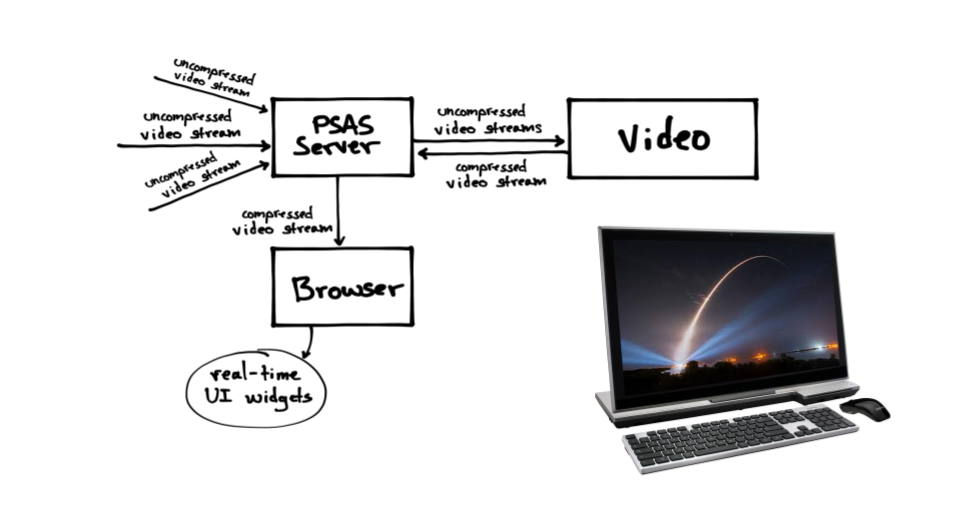
\includegraphics[scale=.4]{./imgs/video.png}
  \end{frame}

  \begin{frame}{Features: Earth Frame View}
    \begin{center}
      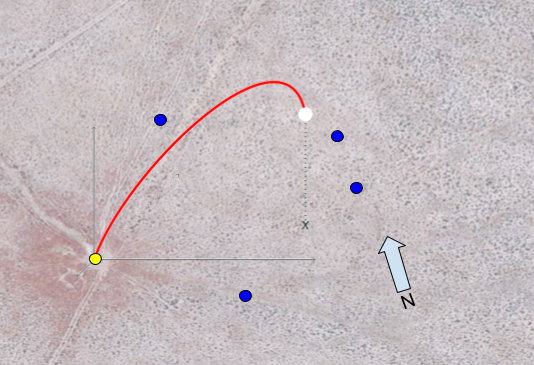
\includegraphics[scale=.5]{./imgs/efv.png}
    \end{center}
  \end{frame}

  \begin{frame}{Features: Vehicle attitude view}
    \begin{center}
      
\includegraphics[scale=.33]{./imgs/attitude.png}
    \end{center}
    \href{https://youtu.be/SqB1a36bGHA}{Video}
  \end{frame}

  \begin{frame}{Features: Telemetry data}
    \begin{center}
      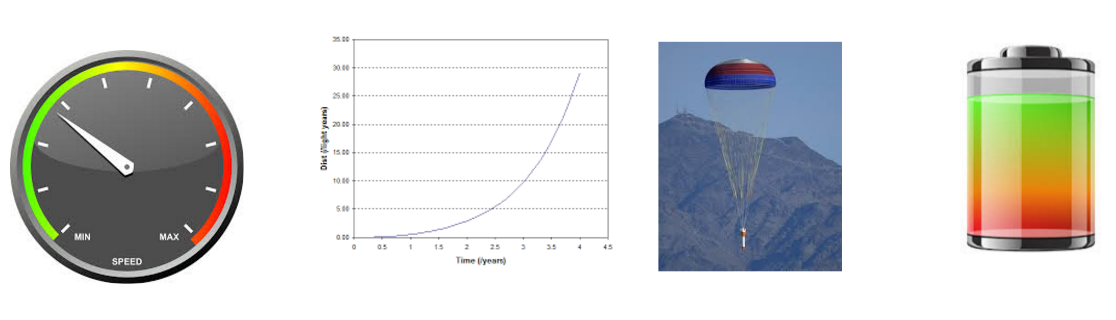
\includegraphics[scale=.45]{./imgs/tel-data.png}
    \end{center}
  \end{frame}


    \begin{frame}{Features: Server}
      \begin{center}
        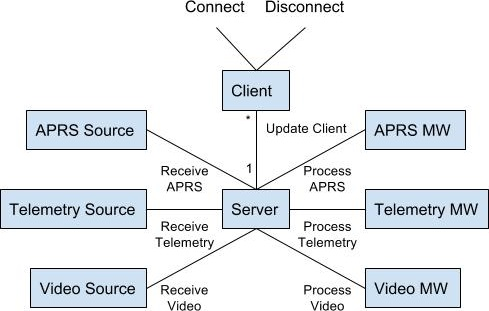
\includegraphics[scale=.7]{./imgs/web-server.jpg}
      \end{center}
    \end{frame}

    \begin{frame}{Features: Instrumentation and logging}
      \begin{itemize}
        \item Purpose
        \begin{itemize}
          \item To facilitate debugging traceability, and configuration
        \end{itemize}
        \item Functionality
        \begin{itemize}
          \item Logs connection status, errors, and relevent events
        \end{itemize}
      \end{itemize}
    \end{frame}



  \begin{frame}[standout]
    \Huge{Assumptions \& Constraints}
  \end{frame}

  \begin{frame}{Process and Schedule}
    \begin{center}
    \begin{tabular}{l c c c}
    Planned Process & Actual Process & Planned Schedule & Actual Schedule \\
    \hline
      {\bf Project Plan} & Same & Weekly & 3 iterations \\

      {\bf Requirements Elicitation} & Same & week 0 to Feb 18th & March 7 \\

      {\bf Risk Plan} & Same & ongoing & ongoing \\

      {\bf SRS/License Agreement} & Same  & Feb 7 - Feb 18  & Feb 7 - March 14 \\

      {\bf SDD} & SDD draft & Feb 18 - March 20 & Feb 21 - March 13 \\

    \end{tabular}
    \end{center}
    Used Trello and GitHub Issues/Milestones/Projects to track tasks
  \end{frame}

    \begin{frame}{Process and Schedule: Term 2}
      \begin{columns}

      \begin{column}{.25\textwidth}
        \begin{block}{Estimated Capacity}
          864 hours

          + 216 hours of slack time

          (96 hours per person)
          \end{block}
        \end{column}


        \begin{column}{.15\textwidth}
          \begin{block}{Back End}
            396 hours
          \end{block}
        \end{column}

        \begin{column}{.01\textwidth}
          \begin{block}{+}
          \end{block}
        \end{column}

        \begin{column}{.15\textwidth}
          \begin{block}{Front End}
            468 hours
          \end{block}
        \end{column}

      \end{columns}
      \bigskip

      With tasks broken down into 1 hour long pieces.
    \end{frame}



  \begin{frame}{Term 1 Deliverables}
    \begin{itemize}
        \item Project Plan
        \item Risk Management Plan
        \item Software Requirements Specification
        \item License Agreement
        \item SDD draft
    \end{itemize}
  \end{frame}

  \begin{frame}[standout]
    \Huge Risk Analysis
  \end{frame}

  \begin{frame}[standout]
    Lessons Learned
  \end{frame}

  \begin{frame}{Lessons: Collaboration with GitHub / Working as a Team}
    \begin{center}
      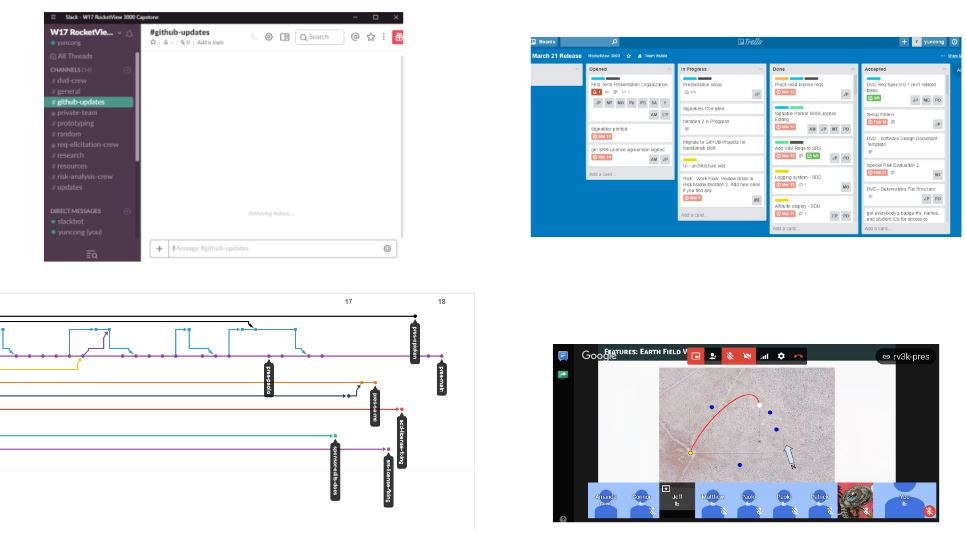
\includegraphics[scale=.45]{./imgs/git.jpg}
    \end{center}
  \end{frame}

  \begin{frame}{Lessons: Working with Sponsors}
    \begin{center}
      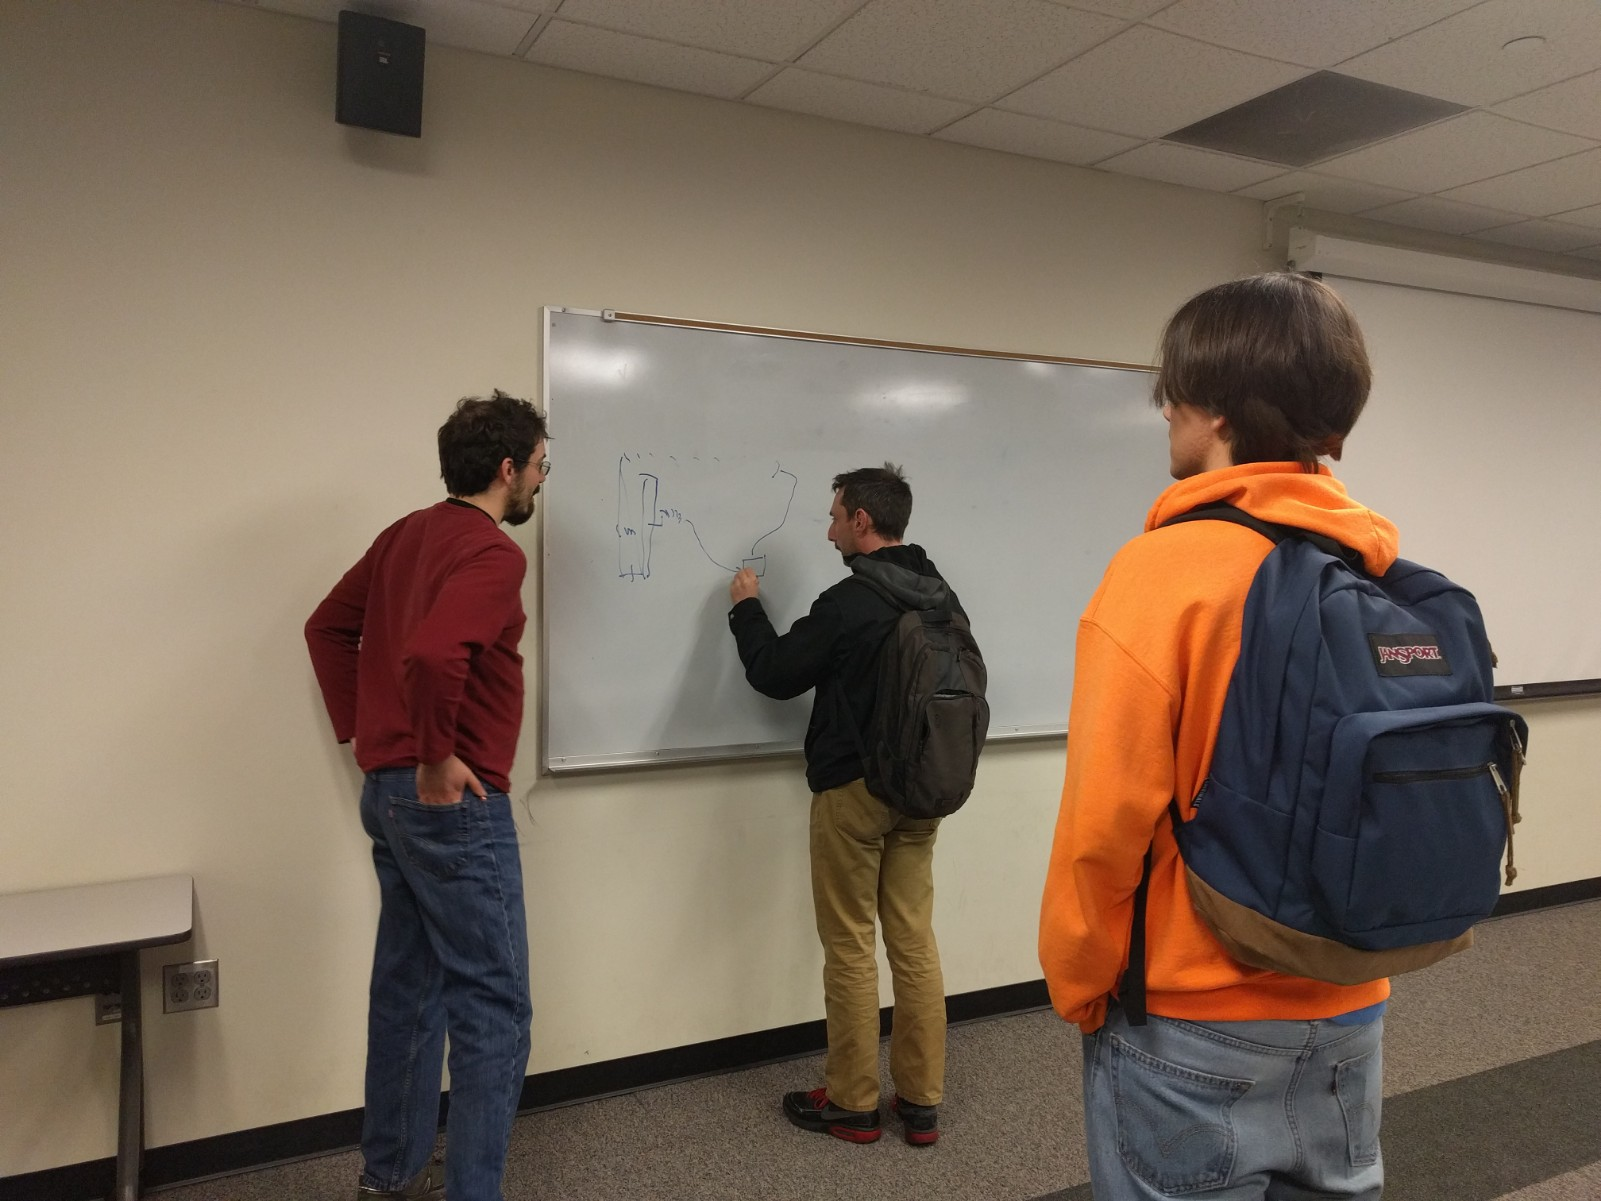
\includegraphics[scale=.15]{./imgs/wws.jpg}
    \end{center}
  \end{frame}

  \begin{frame}{Lessons: PSAS Community}
    \begin{center}
      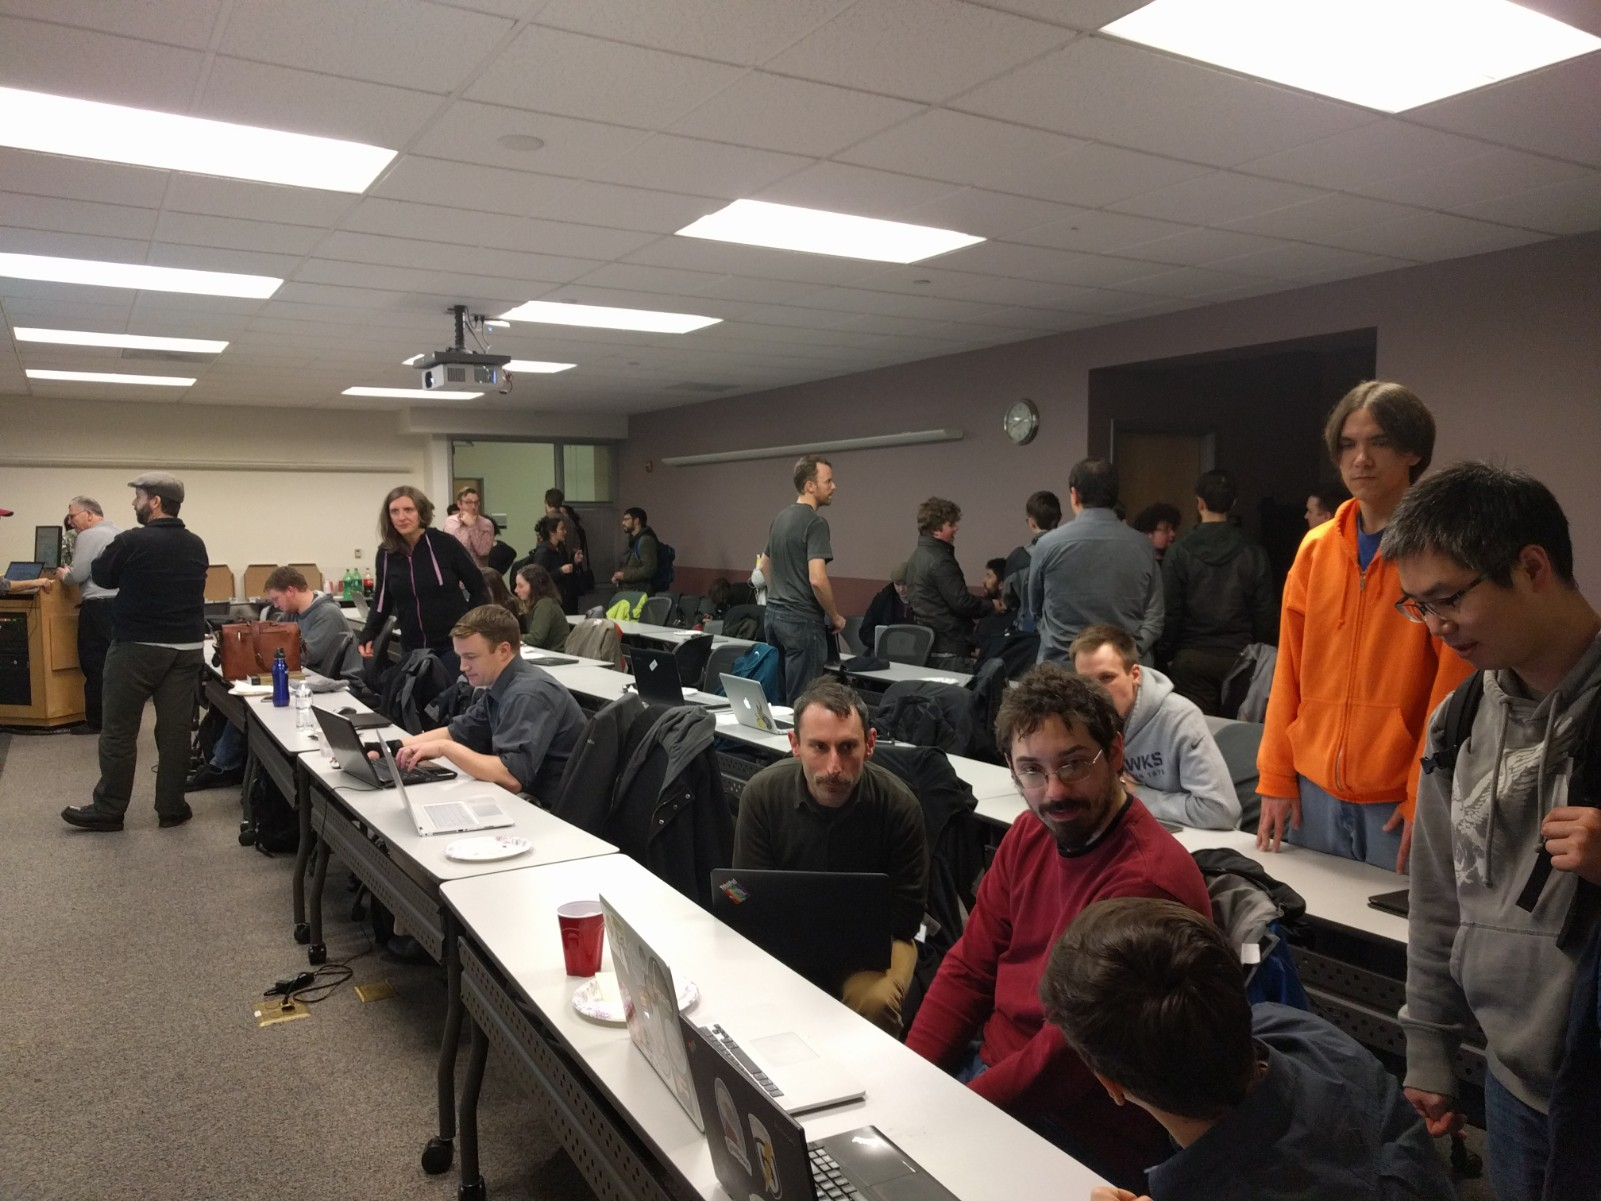
\includegraphics[scale=.15]{./imgs/psas.jpg}
    \end{center}
  \end{frame}
  %\section{amanda-efv}
  % \section{Earth Frame View (EFV) Module}
% TODO: Add Diagram

\subsection{EFV display}
  The Earth Frame display, takes in coordinates, map files, processed trajectory
  data, telemetry data, and recovery crew GPS data. It then outputs browser
  compatible code which renders a 3D map with overlay graphical
  representations of this data in an Earth Frame View.

\subsubsection{3D map rendering}
  The data must be in a form that the map rendering module can easily display.

  Map is rendered from local map files using a JavaScript library (TBD) which
  injects the map into an HTML div element.

\subsubsection{Trajectory path overlay}
  The pre-calculated trajectory is provided in a configuration file by the user.
  This trajectory object is pulled into the EFV module and rendered as an overlay
  on the map.

\subsubsection{Real-time vehicle trajectory location overlay}
  This module takes in the coordinates of the vehicle. The purpose for of the
  GPS data is to indicate the rockets current location on its trajectory.

  The current location of the vehicle is represented as a dot in the EFV display.

\subsubsection{Vehicle path overlay}
  As the vehicle moves on its trajectory path a red trail will be rendered to show
  the trajectory path the vehicle has traveled on.
  The logs the incoming coordinates of the vehicle. This is to insure
  that the rendering can display the path the vehicle has taken.

\subsubsection{Recovery Crew Location Indicator Overlay}
   The system takes in the GPS coordinates of the recovery crews. Earth frame
   view only needs to keep track of the current location of the recovery teams.

\subsubsection{Map angle views}

\subsection{Assets}

\subsubsection{Map files}
  Map files consist of collected terrain maps which are indexed by cartographic
  coordinates.

\subsection{Configuration files}
  Configurable JSON file that stores information about calculated trajectory,
  network ports, and location.

  %The system will display the trajectory of the of where the rocket has been.

  %
  % %\section{seth-mike}
  % \input{VideoProcessing.tex}
  %
  %
  % \section{Rocket Attitude Module}

\subsection{Rocket Attitude Display Module}
The Rocket Attitude display takes in IMU data and a 3D model. It renders this 3D model, and then 
uses IMU data from the rocket to alter the orientation of the model to match that of the live rocket.

\subsubsection{Model Storage}
There is an offline storage which stores the 3D model, as well as the material that is applied to the model.

\subsection{IMU Data Calculations}
The system performs any necessary computations on the IMU data to make it usable for the display module.

\subsubsection{Smoothing Calculations}
The default rotating of the rocket model sometimes causes choppy animation. As a result, the rotating
goes through a smoothing process in order to ensure a smooth display.

\subsection{Display Output}
The module uses a rendered 3D model, along with the processed and smoothed data, to produce a live 
simulation of the real rocket's attitude during its flight.

\begin{figure}[ht!]
\centering
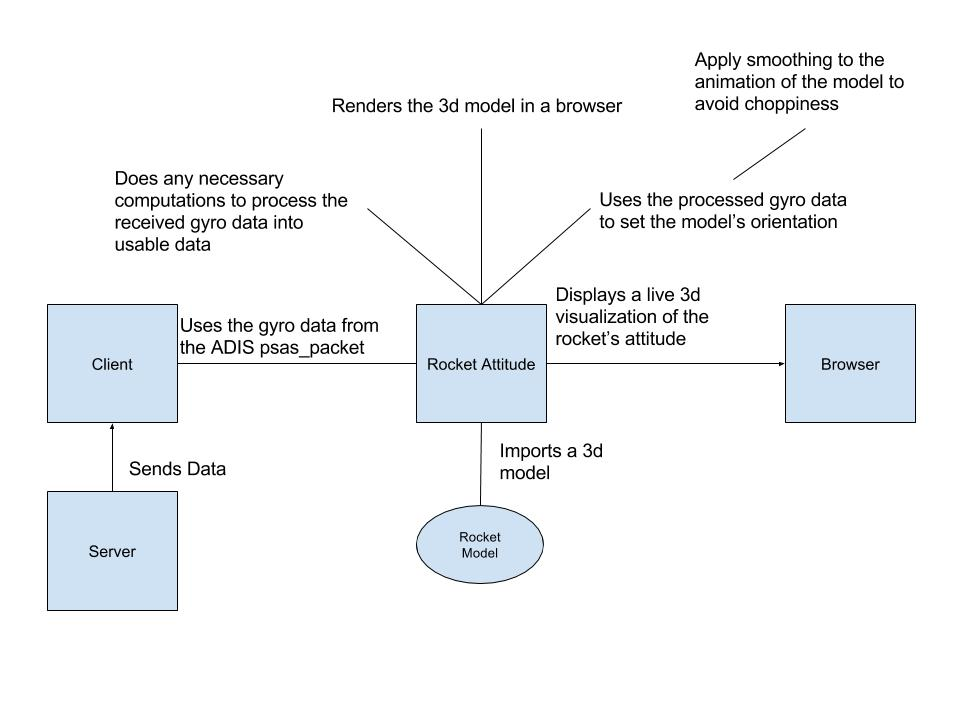
\includegraphics[scale=.4]{imgs/attitude.jpg}
\caption{Rocket Attitude \label{overflow}}
\end{figure}

  %
  % %\input{use-case.tex}
  %
  % \begin{frame}[standout]
  %   \Huge{Use Cases}
  % \end{frame}
  \begin{frame}[standout]
    Thank You!

    \begin{tikzpicture}

      \coordinate (O) at (0,0,0);
      \coordinate (A) at (4,2.5,-2);
      \coordinate (B) at (4,0,-2);
      \draw[->]         (0,0,0) to  (5,0,0)   node[anchor=north east]{};
      \draw[->] (0,0,0) to  (0,3,0)   node[anchor=north east]{};
      \draw[->, dotted] (0,0,0) to  (0,-.5,0) node[anchor=north east]{};
      \draw[->, dotted] (0,0,0) to  (0,0,-5)  node[anchor=east]{};
      \draw[->]         (0,0,0) to  (0,0,1)   node[anchor=east]{};
      \draw[color=red, ultra thick] (O) to [out=70, in=100] (A);
      %\draw[white, thick, dotted, domain=0:5] plot (\x, {0-\x*\x + 5*\x});
      \draw[dotted, thick, ->] (A) to (B) node{$x$};
      %\draw[color=red] (O) to [bend left= 60] (A);
      \draw[color=white, fill=white] (A) circle[radius=.15];
    \end{tikzpicture}

    \Huge{RV3K}
  \end{frame}
\end{document}
